\documentclass[conference,dvipsnames]{IEEEtran}
\IEEEoverridecommandlockouts
% The preceding line is only needed to identify funding in the first footnote. If that is unneeded, please comment it out.
\usepackage{cite}
\usepackage{amsmath,amssymb,amsfonts}
\usepackage{algpseudocode}
\usepackage{graphicx}
\ifCLASSOPTIONcompsoc
  \usepackage[caption=false,font=normalsize,labelfont=sf,textfont=sf]{subfig}
\else
  \usepackage[caption=false,font=footnotesize]{subfig}
\fi
\usepackage{textcomp}
\usepackage{xcolor}
\usepackage{todonotes}
\usepackage{booktabs}
\usepackage{url}
\usepackage{tikz}
\usetikzlibrary{trees, matrix, positioning, patterns, shapes, shadows, shapes.arrows, arrows.meta, shapes.multipart, decorations.pathreplacing, calc, tikzmark, shapes.geometric}
\usepackage{pgfplots}
\pgfplotsset{compat=1.17}
\usepackage{pgf-pie}
\usepackage[binary-units]{siunitx}
\usepackage{mathdots}
\usepackage{mathtools}
\usepackage{bm}
\usepackage{ulem}
\usepackage[colorlinks=true, linkcolor=black, urlcolor=NavyBlue, citecolor=black]{hyperref}

\newcommand{\soutthick}[1]{%
    \renewcommand{\ULthickness}{3pt}%
       \sout{#1}%
    \renewcommand{\ULthickness}{.3pt}% Resetting to ulem default
}

\newcommand{\MatVal}[1]{\bm{\mathit{#1}}}

\def\BibTeX{{\rm B\kern-.05em{\sc i\kern-.025em b}\kern-.08em
    T\kern-.1667em\lower.7ex\hbox{E}\kern-.125emX}}
\begin{document}

\title{\soutthick{Safe}Tix, The Best-Worst QR-Code Ticketing system}

\author{
\IEEEauthorblockN{Julian Partanen and Alexander Mattingley-Scott}
\IEEEauthorblockA{\textit{Beginner's Practical in Binary Hacking, B.Sc. Computer Science} \\
\textit{Heidelberg University, Germany}\\
\href{mailto:me272@uni-heidelberg.de}{me272@uni-heidelberg.de}, \href{mailto:tt249@uni-heidelberg.de}{tt249@uni-heidelberg.de}}
}

\maketitle

\begin{abstract}
	(Optional) Very briefly (two to three sentences) describe your overarching topic
\end{abstract}

% \begin{IEEEkeywords}
% component, formatting, style, styling, insert
% \end{IEEEkeywords}

\section{Your First Question Here}

\subsection{Problem}

Describe the problem the interviewee is expected to solve. If applicable
mention constraints like runtime or memory complexity, coding style, edge
cases, etc. If you use information from external sources,
like~\cite{McDowell_Cracking_2015}, consider a citation if it is a book or
article. For blog entries or other links a footnote with a URL will suffice.

\begin{figure}[h]
    \centering
    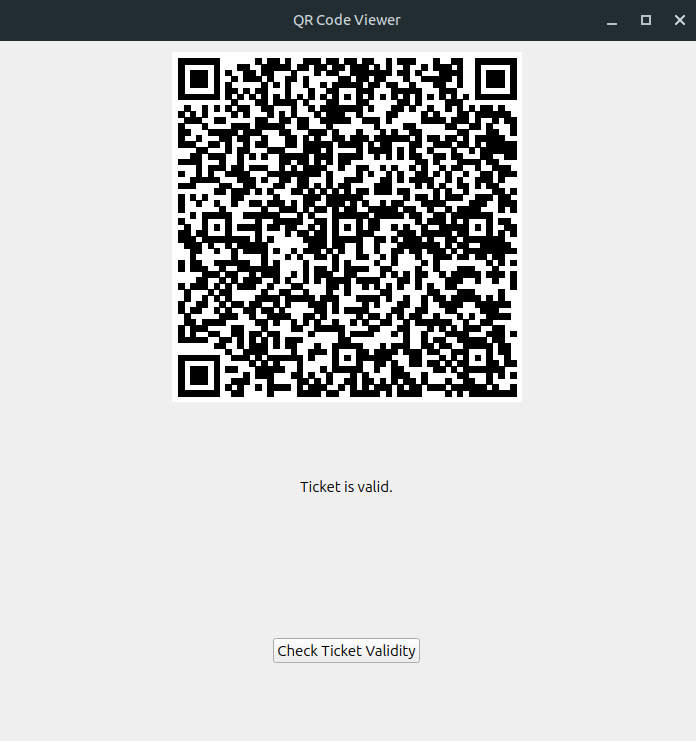
\includegraphics[width=0.44\textwidth]{../figures/QR_Window.png}
    \caption{Example image}
    \label{fig:screenshot}
\end{figure}


\subsection{Baseline Solution}

Give the solution to the previously described problem. Talk about possible
pitfalls and hints you could give the interviewee. Show code snippets where
applicable. You may, of course, also use graphics and plots.

\subsection{(Optional) Post-Interview Experiences}

How was the question received, did interviewees struggle with a particular part
the most.

\section{Your Second Question Here}

See example \texttt{01-question01.tex}.

\section{Your Second Question Here}

See example \texttt{01-question01.tex}.


% Only if you have references
\bibliographystyle{IEEEtran}
\bibliography{bibliography}

\clearpage
%\input{appendix.tex}


\end{document}
